\chapter{Material y métodos}
\label{material_y_metodos}

En esta sección describiremos el trabajo realizado.


\section{Tecnologías empleadas}
En esta sección desglosaremos las tecnologías que utilizaremos
 para realizar el proyecto.

\subsection{Java}
Java es un lenguaje de programación orientado a objetos de propósito general, concurrente,  orientado a objetos que fue diseñado específicamente para tener tan pocas dependencias de implementación como fuera posible. Su intención es permitir que los desarrolladores de aplicaciones escriban el programa una vez y lo ejecuten en cualquier dispositivo (conocido en inglés como WORA, o "write once, run anywhere"), lo que quiere decir que el código que es ejecutado en una plataforma no tiene que ser compilado de nuevo para correr en otra. Java es, a partir de 2012, uno de los lenguajes de programación más populares en uso, particularmente para aplicaciones de cliente-servidor de web, con unos 10 millones de usuarios reportados. \cite{JAVA}
\subsubsection{Mecanismos básicos}
\begin{enumerate}
\item \textbf{Objetos:}
 Es una abstracción encapsulada genérica de datos y los procedimientos para manipularlos.
\item \textbf{Mensajes:}
Los objetos se comunican a través de señales o mensajes, siendo estos mensajes los que hacen que los objetos respondan de diferentes maneras.
\item \textbf{Métodos:}
Es una acción que determina como debe de actuar un objeto cuando recibe un mensaje.
\item \textbf{Clases:}
Es la generalización de un tipo específico de objetos, es decir, es el conjunto de características y comportamientos de todos los objetos que componen la clase.
\end{enumerate}
\subsubsection{Principios fundamentales}
\begin{enumerate}
\item \textbf{Abstracción:}
Es el proceso de representar entidades reales como elementos internos a un programa, la abstracción de los datos es tanto en los atributos, como en los métodos de los objetos.
\item \textbf{Encapsulamiento:}
Cada objeto está aislado del exterior, esta característica permite verlo como una caja negra, que contiene toda la información relacionada con ese objeto. Este aislamiento protege a los datos asociados a un objeto para que no se puedan modificar por quien no tenga derecho a acceder a ellos.
Permite manejar a los objetos como unidades básicas, dejando oculta su estructura interna.
\item \textbf{Herencia:}
Es el medio para compartir en forma automática los métodos y los datos entre las clases y subclases de los objetos. Los objetos heredan las propiedades y el comportamiento de todas las clases a las que pertenece.
\item \textbf{Polimorfismo:}
Esta característica facilita la implementación de varias formas de un mismo método, con lo cual se puede acceder a varios métodos distintos, que tienen el mismo nombre. \cite{JAVA}
\end{enumerate}
\subsubsection{Entornos de funcionamiento}
	
El diseño de Java, su robustez de la industria y su fácil portabilidad han hecho de Java uno de los lenguajes con un mayor crecimiento y amplitud de uso en dispositivos ámbitos de la industria de la informática. Los distintos entornos donde podemos ejecutar una aplicación Java son:
\begin{enumerate}
\item	En dispositivos móviles y sistemas embebidos
\item	En el navegador web
\item	En sistemas de servidor
\item	En aplicaciones de escritorio
\end{enumerate}


\subsection{Android}
Utilizaremos el sistema operativo Android como entorno para implementar 
nuestra aplicación.
Android es un sistema operativo cuyo núcleo está basado en Linux,
 sistema libre, gratuito y multiplataforma. El sistema operativo fue 
desarrollado en Octubre de 2003 por Android Inc., y posteriormente
 comprado por Google en 2005.
Aunque principalmente fue diseñado para dispositivos móviles con
 pantalla táctil como teléfonos inteligentes o tablets, actualmente
también se utiliza para dispositivos wearables, televisiones e incluso
 para automóviles.  

Android permite realizar aplicaciones en un lenguaje basado en Java 
que utiliza como JVM (Java Virtual Machine) ART. Su predecesor es Dalvik~\cite{ART}.


Esta máquina virtual proporciona una serie de mejoras respecto a la jvm habitual de java:
\begin{enumerate}
\item	Compilación AOT (Ahead-of-time): Compila utilizando la herramienta dex2oat.
 Mejora el rendimiento y minimiza el tiempo de instalación de aplicaciones.
\item	Mejora el recolector de basura.
\item	Mejoras para el desarrollo y la depuración:
\begin{enumerate}
\item	Soporta perfiles de pruebas.
\item	Añade nuevas características para depurar, particularmente en el monitor
 de recursos y el recolector de basura.
\item	Mejoras en la descripción de los errores, añadiendo detalles 
como por ejemplo, información relativa a la actividad que intentaba
 realizar antes de un error de tipo java.lang.NullPointerException.
\end{enumerate}
\end{enumerate}

ART nos proporciona un lenguaje de programación con acceso 
de una forma sencilla a las funcionalidades del teléfono 
(como GPS, llamadas, agenda, etc.).

Entre las características más importantes de este sistema operativo,
 es que tiene licencia Open Source, es decir, tanto el código fuente 
como los archivos binarios pueden ser modificados y redistribuidos
 libremente, sin tener que pagar al autor original. Esto lo hace muy
 popular entre fabricantes y desarrolladores, ya que los costes 
disminuyen mucho a la hora de lanzar un teléfono o realizar una aplicación.
	\subsubsection{Arquitectura Android}
En este apartado vamos a ver una visión global por capas de la
 arquitectura empleada por Android. Cada una de estas capas utiliza
 servicios ofrecidos por las anteriores, y ofrece a su vez los suyos 
propios a las capas de niveles superiores, tal y como podemos ver
 en la siguiente figura.
\begin{figure}[h]
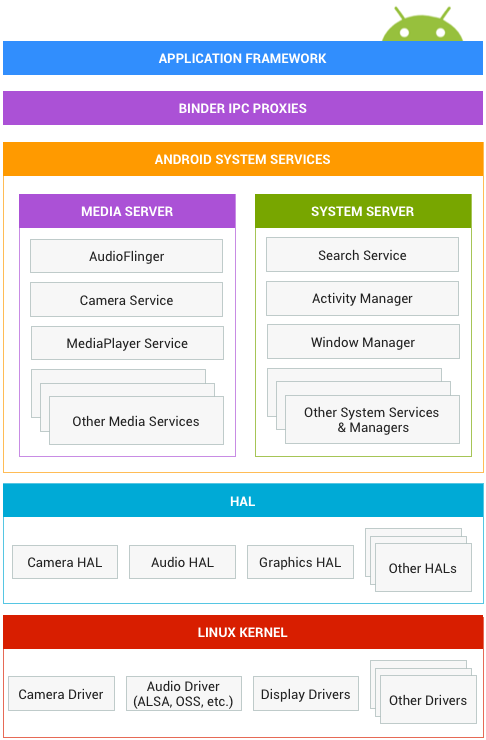
\includegraphics[scale=0.5]{arquitectura_android.png} 
\caption{Arquitectura del sistema Android.}
\end{figure}


\begin{enumerate}
\item	Aplicaciones: Este nivel contiene, tanto las incluidas por defecto 
de Android como aquellas que el usuario vaya añadiendo posteriormente,
 ya sean de terceras empresas o de su propio desarrollo. 
Todas estas aplicaciones utilizan los servicios, las API y
 librerías de los niveles anteriores. 
\item	Framework de Aplicaciones: Representa fundamentalmente el
 conjunto de herramientas de desarrollo de cualquier aplicación. 
Toda aplicación que se desarrolle para Android, ya sean las propias 
del dispositivo, las desarrolladas por Google o terceras compañías,
 o incluso las que el propio usuario cree, utilizan el mismo conjunto
 de API y el mismo ``framework'', representado por este nivel. 
Entre las API más importantes ubicadas aquí, se pueden encontrar las siguientes:
\begin{enumerate}
\item	Activity Manager: Conjunto de API que gestiona el ciclo de vida de
 las aplicaciones en Android.
\item	Window Manager: Gestiona las ventanas de las aplicaciones y
 utiliza la librería Surface Manager.
\item	Content Provider: Permite a cualquier aplicación compartir sus
 datos con las demás aplicaciones de Android. Por ejemplo, gracias a 
esta API la información de contactos, agenda, mensajes, etc. 
será accesible para otras aplicaciones.
\item	View System: Proporciona un gran número de elementos para poder
 construir interfaces de usuario (GUI), como listas, mosaicos, 
botones, ``check-boxes'', tamaño de ventanas, control de las
 interfaces mediante teclado, etc. Incluye también algunas vistas
 estándar para las funcionalidades más frecuentes.
\item	Notification Manager: Mediante el cual las aplicaciones,
 usando un mismo formato, comunican al usuario eventos que
 ocurran durante su ejecución: una llamada entrante, un mensaje recibido,
 conexión Wifi disponible, ubicación en un punto determinado, etc. 
Si llevan asociada alguna acción, en Android denominada Intent,
(por ejemplo, atender una llamada recibida) ésta se activa mediante un simple clic.
\item	Package Manager: Permite obtener información sobre los
 paquetes instalados en el dispositivo Android, además de
 gestionar la instalación de nuevos paquetes.
\item	Telephone Manager: Incluye todas las API vinculadas
 a las funcionalidades propias del teléfono (llamadas, mensajes, etc.).
\item	Resource Manager: Permite gestionar los elementos
 (cadenas de texto traducidas a diferentes idiomas, imágenes, sonidos o layouts)
 que forman parte de la aplicación y que están fuera del código.
\item	Location Manager: Posibilita a las aplicaciones la obtención
 de información de localización y posicionamiento.
\end{enumerate}
\item XMPP Service: Colección de API para utilizar este protocolo
 de intercambio de mensajes basado en XML. 
\item	Librerías: La siguiente capa se corresponde con las librerías
 utilizadas por Android. Estas han sido escritas utilizando C/C++ y
 proporcionan a Android la mayor parte de sus capacidades 
más características. Junto al núcleo basado en Linux, estas librerías 
constituyen el corazón de Android.
Entre las librerías más importantes ubicadas aquí, se pueden
 encontrar las siguientes:
\begin{enumerate}
\item	Surface Manager: Es la encargada de componer los 
diferentes elementos de navegación de pantalla. Gestiona
 también las ventanas pertenecientes a las distintas
 aplicaciones activas en cada momento.
\item	Media Framework: Proporciona todos los códecs necesarios 
para el contenido multimedia soportado en Android (vídeo, audio,
 imágenes estáticas y animadas, etc.)
\item	SQLite: Creación y gestión de bases de datos relacionales.
\item	OpenGL/SL y SGL: Representan las librerías gráficas y,
 por tanto, sustentan la capacidad gráfica de Android.
 OpenGL/SL maneja gráficos en 3D y permite utilizar,
 en caso de que esté disponible en el propio dispositivo móvil,
 el hardware encargado de proporcionar gráficos 3D.
 Por otro lado, SGL proporciona gráficos en 2D,
 por lo que será la librería más habitualmente utilizada por
 la mayoría de las aplicaciones. Una característica importante
 de la capacidad gráfica de Android es que es posible 
desarrollar aplicaciones que combinen gráficos en 3D y 2D.
\item	FreeType: Permite trabajar de forma rápida y
 sencilla con distintos tipos de fuentes.
\item	WebKit: Proporciona un motor para las aplicaciones
 de tipo navegador y forma el núcleo del actual navegador
 incluido por defecto en la plataforma Android.
\item	SSL: Posibilita la utilización de dicho protocolo para
 establecer comunicaciones seguras.
\item	Libc: Incluye todas las cabeceras y funciones según
 el estándar del lenguaje C. Todas las demás librerías se 
definen en este lenguaje.
\end{enumerate}
\item	Tiempo de ejecución de Android: Al mismo nivel que las
 librerías de Android se sitúa el entorno de ejecución.
 Éste lo constituyen las Core Libraries, que son librerías con
 multitud de clases Java y la máquina virtual ART~\cite{ART}.
\item Núcleo Linux: Android utiliza el núcleo de Linux como una 
capa de abstracción para el hardware disponible en los dispositivos
 móviles. Esta capa contiene los drivers necesarios para que cualquie
r componente hardware pueda ser utilizado mediante las llamadas
 correspondientes. Siempre que un fabricante incluye un nuevo
 elemento de hardware, lo primero que se debe realizar para que 
pueda ser utilizado desde Android es crear las librerías de control
 o drivers necesarios dentro de este kernel de Linux embebido 
en el propio Android. 
\end{enumerate}
\subsubsection{Componentes Android}
Existen cinco componentes importantes en las aplicaciones Android:

\begin{figure}[h]
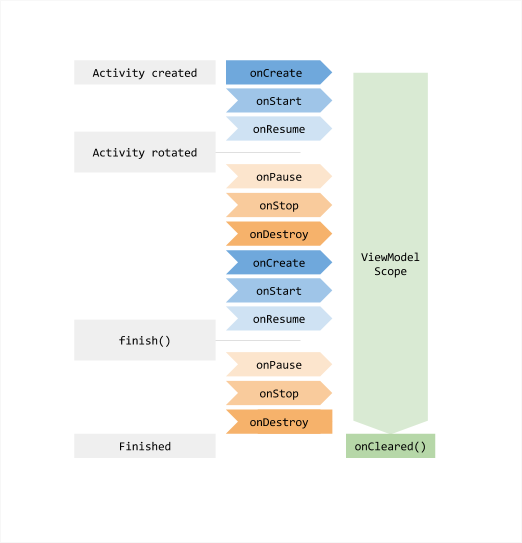
\includegraphics[scale=0.50]{ciclo_de_vida.png} 
\caption{Ciclo de vida de una aplicación Android.}
\end{figure}
\begin{enumerate}

\item	Activity: Se puede decir que una actividad es cada una de
 las pantallas que nosotros mostramos en la ejecución de nuestra 
aplicación. Cada actividad puede encontrarse en diferentes estados:
\begin{enumerate}
\item	onCreate: Representa el momento en que se crea la actividad.
\item	onStart: Es donde la actividad se muestra en pantalla.
\item	onRestart: Cuando una aplicación estaba parada y la volvemos a activar.
\item	onResume: La actividad va a empezar a responder a la interacción del usuario.
\item	onPause: La actividad va a dejar de responder a la interacción del usuario.
\item	onStop: Cuando la actividad pasa a segundo plano.
\item	onDestroy: Cuando se destruye una actividad y se liberan sus recursos.
\end{enumerate}




Una actividad consta de dos partes:
\begin{enumerate}
\item	La parte lógica: se trata de un archivo java donde se manipula,
 interactúa y coloca el código de la actividad.
\item	La parte gráfica: Se trata de un XML donde se introducen los
 elementos que formarán la estructura de la pantalla.
\end{enumerate}
\item	Services: Son tareas que se ejecutan en segundo plano y no
 tienen una interfaz que vea el usuario. Se suelen utilizar para realizar 
operaciones de larga ejecución o para realizar trabajo con procesos remotos.
Se encargan de realizar tareas que deben continuar ejecutándose 
cuando nuestra aplicación no está en primer plano.
\item	Content Provider: Se trata de un mecanismo proporcionado
 por la plataforma Android para permitir compartir información entre 
aplicaciones. Se permite acceder al sistema de ficheros, bases de 
datos SQLite, la información se encuentran la lista de contactos, la 
aplicación de SMS, o el calendario/agenda.  
\item	Intent: Son objetos que se utilizan para arrancar actividades o 
servicios, o enviar eventos a múltiples destinatarios. Estos objetos 
también se pueden utilizar para realizar paso de mensajes entre 
actividades de la misma aplicación o entre distintas aplicaciones.
\item Broadcast Receiver: Un broadcast es un mensaje que cualquiera 
aplicación puede recibir. Estos mensajes broadcast pueden ser 
un reinicio del dispositivo, aviso de batería baja o al conectar el
 móvil a un cargador. Con este componente se puede configurar
 el recibir ese broadcast y que nuestra aplicación haga alguna acción 
determinada en ese momento.
\end{enumerate}
\subsubsection{Estructura de una aplicación Android}
En este apartado vamos a explicar la estructura de los componentes
 que tiene una aplicación Android.
\begin{enumerate}
\item	Src: En esta carpeta se introducen los archivos java 
que componen nuestra aplicación.
\item	Gen: Dentro de esta carpeta hay un archivo llamado ``R.java'' 
donde se guardan los identificadores de todos los componentes
 utilizados en la aplicación.
\item	Libs: Se encuentran librerías externas que necesita el proyecto.
\item	Res: En este directorio se encuentran todos los recursos
 de la aplicación.
\item	Res/drawable: En esta carpeta se guardan las imágenes 
que vamos a utilizar en nuestra aplicación.
\item	Res/layout: Carpeta donde se guardan los XML de las actividades.
\item	Res/values: Carpeta donde se guarda el archivo ``strings.xml'',
 el cual almacena las cadenas de texto que utilizaremos en la aplicación. 
AndroidManifest.xml: Este archivo es el más importante de la aplicación
 y por eso le vamos a dedicar un pequeño apartado para profundizar más en él.
\subsubsection{Android Manifest}
Éste archivo se considera el más importante de la aplicación ya que es
 donde se declaran todas las actividades de la aplicación, los permisos,
 versiones del SDK que usamos, etc.
 
En la primera línea se indica la versión y el formato del documento:
 
La etiqueta principal es <manifest> y tiene varios atributos:
\begin{enumerate}
\item[Xmlns]: lo coloca Eclipse por defecto.
\item[Package]: Hace referencia al nombre del paquete de la aplicación.
\item[VersionCode]: Es el número de versión del código de la aplicación.
\item[VersionName]: También es el número de la versión.
 \end{enumerate}
 
La etiqueta SDK se configura para saber la compatibilidad de las 
versiones en Android.
\begin{enumerate}
\item minSDKVersion: Indica la versión mínima de SDK para que funcione
 nuestra aplicación.
\item targetSdkVersion: Es la versión de la API a la que se dirige
 principalmente la aplicación.
\end{enumerate}
La etiqueta <uses-permission>~se utiliza para dar permisos a la aplicación.
En nuestro caso, hemos configurado para que nuestra aplicación
pueda acceder a internet, pueda acceder al GPS y pueda escribir 
en un almacenamiento externo.
 
Dentro de la etiqueta <application> se introducen todos los 
elementos que componen la aplicación.
\begin{enumerate}
\item allowBackup: Con el valor ``true'' se le permite al sistema 
hacer copia de seguridad de la aplicación y del contenido.
\item Icon: Es el icono de la aplicación.
\item Label: Es el nombre de la aplicación.
\item Theme: Es el estilo de la aplicación.
\end{enumerate}
En la etiqueta <activity> es donde se dan de alta todas las 
actividades que vamos a tener en la aplicación.
\begin{enumerate}
\item Name: Contiene el nombre de la clase java que implementa el activity.
\item Label: Es el nombre de la activity.
\end{enumerate}
<Intent-filter> indica lo que la activity tiene permitido hacer.
\end{enumerate}


\subsection{Sistema de posicionamiento global}
Utilizaremos el sistema GPS para localizar el dispositivo móvil en el agua.

A continuación describiremos brevemente en que se base este sistema.

El Sistema de Posicionamiento Global (en inglés, GPS; Global Positioning System)
, y originalmente Navstar GPS, es un sistema que permite determinar
 en toda la Tierra la posición de un objeto (una persona, un vehículo)
 con una precisión de hasta centímetros (si se utiliza GPS diferencial), 
aunque lo habitual son unos pocos metros de precisión. El sistema fue
 desarrollado, instalado y empleado por el Departamento de Defensa
 de los Estados Unidos. Para determinar las posiciones en el globo, 
el sistema GPS se sirve de 24 a 32 satélites y utiliza la trilateración.

El GPS funciona mediante una red de como mínimo 24 satélites en
 órbita sobre el planeta Tierra, a 20 180 km de altura, con trayectorias 
sincronizadas para cubrir toda la superficie de la Tierra. Cuando
 se desea determinar la posición tridimensional, el receptor que se 
utiliza para ello localiza automáticamente como mínimo cuatro satélites 
de la red, de los que recibe unas señales indicando la identificación 
y hora del reloj de cada uno de ellos, además de información sobre 
la constelación. Con base en estas señales, el aparato sincroniza el 
reloj del GPS y calcula el tiempo que tardan en llegar las señales al 
equipo, y de tal modo mide la distancia al satélite mediante el método 
de trilateración inversa, el cual se basa en determinar la distancia
 de cada satélite al punto de medición. Conocidas las distancias, 
se determina fácilmente la propia posición relativa respecto a los
 satélites. Conociendo además las coordenadas o posición de cada
 uno de ellos por la señal que emiten, se obtiene la posición absoluta
 o coordenadas reales del punto de medición. También se consigue
 una gran exactitud en el reloj del GPS, similar a la de los relojes
 atómicos que lleva a bordo cada uno de los satélites.

\subsubsection{Funcionamiento}

La información que es útil al receptor GPS para determinar su
 posición se llama efemérides. En este caso cada satélite emite
 sus propias efemérides, en la que se incluye la salud del satélite, 
su posición en el espacio, su hora atómica, información doppler, etc.

Mediante la trilateración se determina la posición del receptor:
\begin{itemize}

\item Cada satélite indica que el receptor se encuentra en un punto
 en la superficie de la esfera, con centro en el propio satélite y 
de radio la distancia total hasta el receptor.
\item Obteniendo información de dos satélites queda determinada
 una circunferencia que resulta cuando se intersecan las dos esferas 
en algún punto de la cual se encuentra el receptor.
\item Teniendo información de un tercer satélite, se elimina el 
inconveniente de la falta de sincronización entre los relojes de los
 receptores GPS y los relojes de los satélites. Y es en este momento 
cuando el receptor GPS puede determinar una posición 3D exacta
 (latitud, longitud y altitud).
\end{itemize}
\subsubsection{Integración con telefonía móvil}
Actualmente dentro del mercado de la telefonía móvil la tendencia 
es la de integrar, por parte de los fabricantes, la tecnología GPS 
dentro de sus dispositivos. El uso y masificación del GPS está 
particularmente extendido en los teléfonos móviles smartphone, lo que
 ha hecho surgir todo un ecosistema de software para este tipo de
 dispositivos, así como nuevos modelos de negocios que van desde el
 uso del terminal móvil para la navegación tradicional punto-a-punto 
hasta la prestación de los llamados Servicios Basados en la Localización (LBS).

Un buen ejemplo del uso del GPS en la telefonía móvil son las 
aplicaciones que permiten conocer la posición de amigos cercanos
sobre un mapa base. Para ello basta con tener la aplicación
 respectiva para la plataforma deseada (Android, Bada, IOS, WP, Symbian)
 y permitir ser localizado por otros.

\footnote{Fuente : GPS~\cite{GPS}}

\subsection{JSON}
\label{json}
JSON (JavaScript Object Notation - Notación de Objetos de JavaScript) 
es un formato ligero de intercambio de datos. Leerlo y escribirlo es simple
 para humanos, mientras que para las máquinas es simple interpretarlo y 
generarlo. Está basado en un subconjunto del Lenguaje de Programación
 JavaScript. JSON es un formato de texto que es completamente independiente
 del lenguaje pero utiliza convenciones que son ampliamente conocidos por los
 programadores de la familia de lenguajes C, incluyendo C, C++, Java, 
JavaScript, Perl, Python, y muchos otros. Estas propiedades hacen que 
JSON sea un lenguaje ideal para el intercambio de datos.

JSON está constituído por dos estructuras:
\begin{enumerate}

\item Una colección de pares de nombre/valor. En varios lenguajes 
esto es conocido como un objeto, registro, estructura, diccionario, 
tabla hash, lista de claves o un arreglo asociativo.
\item Una lista ordenada de valores. En la mayoría de los lenguajes, 
esto se implementa como arreglos, vectores, listas o sequencias.
\end{enumerate}
Estas son estructuras universales; virtualmente todos los lenguajes 
de programación las soportan de una forma u otra. Es razonable que
 un formato de intercambio de datos que es independiente del lenguaje 
de programación se base en estas estructuras.

\footnote{Fuente :JSON~\cite{JSON}}

\subsection{Firebase}
Firebase es una plataforma para el desarrollo de aplicaciones web y
 aplicaciones móviles. Firebase se integra actualmente con otros
 servicios de Google para poder ofrecer productos a mayor escala
 para los desarrolladores.
Los servicios ofrecidos por Firebase son los siguientes: 
\begin{enumerate}
\item \textbf{Firebase Analytics: } es una aplicación
 gratuita que proporciona una visión profunda sobre el
 uso de la aplicación por parte de los usuarios.
\item \textbf{Firebase Cloud Messaging: }
Antiguamente conocido como Google Cloud Messaging (GCM),
 Firebase Cloud Messaging (FCM) es una plataforma para mensajes 
y notificaciones para Android, iOS, y aplicaciones web que
 actualmente puede ser usada de forma gratuita.
\item \textbf{Firebase Auth:} es un servicio que puede autenticar
 los usuarios utilizando únicamente código del lado del cliente.
 Incluye la autenticación mediante Facebook, GitHub, Twitter y 
Google. Además, incluye un sistema de administración del usuario
 por el cual los desarrolladores pueden habilitar la autenticación de
 usuarios con email y contraseña que se almacenarán en Firebase.
\item \textbf{Realtime Database:}
Firebase proporciona una base de datos en tiempo real y back-end.
 El servicio proporciona a los desarrolladores de aplicaciones una API
 que permite que la información de las aplicaciones sea sincronizada
 y almacenada en la nube de Firebase. La compañía habilita integración
 con aplicaciones Android, iOS, JavaScript, Java, Objective-C, Swift
 y Node.js. La base de datos es también accesible a través de una 
REST API e integración para varios sistemas de Javascript como
 AngularJS, React, Ember.js y Backbone.js.La REST API utiliza el 
protocolo SSE (del inglés Server-Sent Events), el cual es una API
 para crear conexiones de HTTP para recibir notificaciones push 
de un servidor.
\item \textbf{Firebase Storage:} proporciona cargas y descargas
 seguras de archivos para aplicaciones Firebase, sin importar la 
calidad de la red. El desarrollador lo puede utilizar para almacenar
 imágenes, audio, vídeo, o cualquier otro contenido generado por
 el usuario. Firebase Storage se basa en el almacenamiento de
 Google Cloud Storage.
\item \textbf{Firebase Firestore:} es un servicio derivado de 
Google Cloud Platform, adaptado a la plataforma de Firebase.
 Al igual que Realtime Database, es una base de datos NoSQL,
 aunque presenta diversas diferencias. Se organiza en forma 
de documentos agrupados en colecciones, y en ellos se pueden
 incluir tanto campos de diversos tipos (cadenas de texto, números,
 puntos geográficos, referencias a la propia base de datos, arrays,
 booleanos, marcas de tiempo, e incluso objetos propios) como 
otras subcolecciones.
\end{enumerate}

Utilizaremos Realtime Database ya que nos ofrece la estabilidad 
de un producto muy probado y usado y muy baja latencia, por lo
 que es una excelente opción para la sincronización frecuente de 
estados.

\subsubsection{Bases de datos no relacionales NoSQL}

Empezamos definiendo el concepto de base de datos no relacionales NoSQL.

Pese a la no existencia de una definición formal, cuando hablamos de base datos NoSQL nos referimos a una amplia clase de sistemas de gestión de datos (mecanismos para el almacenamiento y recuperación de datos) que difieren, en aspectos importantes, del modelo clásico de relaciones entre entidades (o tablas) existente en los sistemas de gestión bases de datos relacionales, siendo el más destacado el que no usan SQL como lenguaje principal de consulta.
Aunque son conocidas desde la década de los 60 del pasado siglo, su auge actual viene determinado por el uso que, de estos sistemas han hecho las principales compañías de internet como Amazon, Google, Twitter y Facebook. Estas compañías tenían que enfrentarse a nuevos desafíos en el tratamiento de los datos motivados por el enorme crecimiento de la Web donde se requería dar respuesta a la necesidad de proporcionar información procesada a partir de grandes volúmenes de datos con unas estructuras horizontales, más o menos, similares y con aplicaciones web que debían dar respuesta a las peticiones de un número elevado e indeterminado de usuarios en el menor tiempo posible. Estas compañías se dieron cuenta de que el rendimiento y sus necesidades de tiempo real eran más importantes que la consistencia de los datos, aspecto este último al que las bases de datos relacionales tradicionales dedicaban una gran cantidad de tiempo de proceso.

Las características comunes entre todas las implementaciones de bases de datos NoSQL suelen ser las siguientes:
\begin{enumerate}
\item \textbf{Consistencia Eventual:} A diferencia de las bases de datos relacionales tradicionales, en la mayoría de sistemas NoSQL, no se implementan mecanismos rígidos de consistencia que garanticen que cualquier cambio llevado a cabo en el sistema distribuido sea visto, al mismo tiempo, por todos los nodos y asegurando, también, la no violación de posibles restricciones de integridad de los datos u otras reglas definidas. En su lugar y para obtener un mayor rendimiento, se ofrece el concepto de "consistencia eventual", en el que los cambios realizados "con el tiempo" serán propagados a todos los nodos por lo que, una consulta podría no devolver los últimos datos disponibles o proporcionar datos inexactos, problema conocido como lecturas sucias u obsoletas.
Asimismo, en algunos sistemas NoSQL se pueden presentar perdidas de datos en escritura. Esto se conoce también como BASE (Basically Available Soft-state Eventual Consistency), en contraposición a ACID (Atomicity, Consistency, Isolation, Durability), su analogía en las bases de datos relacionales.
\item \textbf{Flexibilidad en el esquema:} En la mayoría de base de datos NoSQL, los esquemas de datos son dinámicos; es decir, a diferencia de las bases de datos relacionales en las que, la escritura de los datos debe adaptarse a unas estructuras(o tablas, compuestas a su vez por filas y columnas) y tipos de datos pre-definidos, en los sistemas NoSQL, cada registro (o documento, como se les suele llamar en estos casos) puede contener una información con diferente forma cada vez, pudiendo así almacenar sólo los atributos que interesen en cada uno de ellos, facilitando el polimorfismo de datos bajo una misma colección de información. También se pueden almacenar estructuras complejas de datos en un sólo documento, como por ejemplo almacenar la información sobre una publicación de un blog (título, cuerpo de texto, autor, etc) junto a los comentarios y etiquetas vertidos sobre el mismo, todo en un único registro.
\item \textbf{Escalabilidad horizontal:} Por escalabilidad horizontal se entiende la posibilidad de incrementar el rendimiento del sistema añadiendo, simplemente, más nodos (servidores) e indicando al sistema cuáles son los nodos disponibles.
\item \textbf{Estructura distribuida:} Generalmente los datos se distribuyen, entre los diferentes nodos que componen el sistema. Hay dos estilos de distribución de datos:
\begin{enumerate}
\item \textbf{Particionado (ó Sharding):} El particionado distribuye los datos entre múltiples servidores de forma que, cada servidor, actúe como única fuente de un subconjunto de datos. Normalmente, a la hora de realizar esta distribución, se utilizan mecanismos de tablas de hash distribuidas (DHT). 
\item \textbf{Réplica:} La réplica copia los datos entre múltiples servidores, de forma que cada bit de datos pueda ser encontrado en múltiples lugares. Esta réplica puede realizarse de dos maneras:
Réplica maestro-esclavo en la que un servidor gestiona la escritura de la copia autorizada mientras que los esclavos se sincronizan con este servidor maestro y sólo gestionan las lecturas.
Réplica peer-to-peer en la que se permiten escrituras a cualquier nodo y ellos se coordinan entre sí para sincronizar sus copias de los datos
\end{enumerate}
\item \textbf{Tolerancia a fallos y Redundancia: } Pese a lo que cualquiera pueda pensar cuando se habla de NoSQL, no todas las tecnologías existentes bajo este paraguas usan el mismo modelo de datos ya que, al ser sistemas altamente especializados, la idoneidad particular de una base de datos NoSQL dependerá del problema a resolver. Así a todo, podemos agrupar los diferentes modelos de datos usados en sistemas NoSQL en cuatro grandes categorías:
\begin{enumerate}
\item \textbf{Base de datos de Documentos: } Este tipo de base de datos almacena la información como un documento, usando para habitualmente para ello una estructura simple como JSON, BSON o XML y donde se utiliza una clave única para cada registro. Este tipo de implementación permite, además de realizar búsquedas por clave–valor, realizar consultas más avanzadas sobre el contenido del documento. Son las bases de datos NoSQL más versátiles.
\item \textbf{Almacenamiento Clave-Valor:} Son el modelo de base de datos NoSQL más popular, además de ser la más sencilla en cuanto a funcionalidad. En este tipo de sistema, cada elemento está identificado por una clave única, lo que permite la recuperación de la información de forma muy rápida, información que suele almacenarse como un objeto binario. Se caracterizan por ser muy eficientes tanto para las lecturas como para las escrituras. 
\item \textbf{Bases de datos de grafos:} Usadas para aquellos datos cuyas relaciones se pueden representar adecuadamente mediante un grafo. Los datos se almacenan en estructuras grafo con nodos (entidades), propiedades (información entre entidades) y líneas (conexiones entre las entidades). 
\item \textbf{Base de datos Columnar (o Columna ancha):} En vez de tablas, en las bases de datos de columna tenemos familias de columnas que, son los contenedores de las filas. A diferencia de los RDBMS, no necesita conocer de antemano todas las columnas, cada fila no tiene por qué tener el mismo número de columnas. Este tipo de bases de datos se adecuan mejor a operaciones analíticas sobre grandes conjuntos de datos.
\end{enumerate}

\end{enumerate}
Pese a todas las opciones proporcionadas por el auge de las bases de datos NoSQL, esto no significa la desaparición de las bases de datos de RDBMS ya que son tecnologías complementarias. Estamos entrando en una era de persistencia políglota, una técnica que utiliza diferentes tecnologías de almacenamiento de datos para manejar las diversas necesidades de almacenamiento de datos. Hemos elegido la implementación de una base de datos NoSQL para nuestra aplicación ya que para nosotros el rendimiento es más importante que preservar el modelo relacional. Además de la posibilidad de escalar de forma sencilla, hemos tenido en cuenta otros criterios: 
\begin{enumerate}
\item El volumen de lecturas y escrituras
\item Tolerancia por datos inconsistentes en réplicas
\item La naturaleza de las relaciones entre entidades y cómo eso afecta los patrones de consulta
\item Disponibilidad y requisitos de recuperación de desastres
\item La necesidad de flexibilidad en los modelos de datos
\item Requisitos de latencia
\end{enumerate}
\subsubsection{Bases de datos no relacionales NoSQL}
Nos vamos a decantar por un modelo Almacenamiento Clave-Valor y vamos a almacenar una lista de estructuras JSON.
\\
Este tipo de bases de datos Clave-Valor se utilizan en una amplia gama de aplicaciones, como las siguientes:
\begin{enumerate}
\item Almacenamiento en caché de datos de bases de datos relacionales para mejorar el rendimiento
\item Seguimiento de atributos transitorios en una aplicación web, como un carrito de compras
\item Almacenamiento de configuración e información de datos de usuario para aplicaciones móviles
\item Almacenar objetos grandes, como imágenes y archivos de audio
\end{enumerate}
\footnote{Fuente: Oracle \cite{DEFINICIONNOSQL} y NoSQL for mere mortals \cite{NOSQL}}



\subsubsection{Firebase Realtime Database}
Firebase Realtime Database es una base de datos alojada en la nube que nos permitirá almacenar y sincronizar datos. Los datos se sincronizan con todos los clientes en tiempo real y se mantienen disponibles cuando la app no tiene conexión.
\\

Los datos se almacenan en formato JSON y se sincronizan en tiempo real con cada cliente conectado. Cuando compilas apps multiplataforma con el SDK de iOS, Android y JavaScript, todos los clientes comparten una instancia de Realtime Database y reciben actualizaciones automáticamente con los datos más recientes.
\\

Las funciones clave que nos proporciona son las siguientes:

\begin{enumerate}

\item \textbf{Tiempo real:}
En lugar de solicitudes típicas de HTTP, Firebase Realtime Database usa la sincronización de datos (cada vez que cambian los datos, los dispositivos conectados reciben esa actualización en milisegundos). Proporciona experiencias colaborativas y envolventes sin pensar en el código de red.
\item \textbf{Sin conexión:}
Las apps Firebase continúan respondiendo, incluso sin conexión, dado que el SDK de Firebase Realtime Database hace que tus datos persistan en el disco. Cuando se restablece la conexión, el dispositivo cliente recibe los cambios que faltaban y los sincroniza con el estado actual del servidor.
\item \textbf{Acceso desde dispositivos cliente:}
Se puede acceder a Firebase Realtime Database directamente desde un dispositivo móvil o un navegador web; no se necesita un servidor de aplicaciones. La seguridad y la validación de datos están disponibles a través de las reglas de seguridad de Firebase Realtime Database: reglas basadas en expresiones que se ejecutan cuando se leen o se escriben datos.
\item \textbf{Escalamiento en varias bases de datos:}
Con Firebase Realtime Database, puedes satisfacer las necesidades de datos de la app a gran escala: podrás dividir la información en diversas instancias de bases de datos dentro del mismo proyecto de Firebase. Usa Firebase Authentication para optimizar el proceso de autenticación en el proyecto. Podrás autenticar a usuarios en varias instancias de la base de datos. Controla el acceso a la información de cada base de datos. Para ello, usa las reglas personalizadas de Firebase Realtime Database en cada una de las instancias de la base de datos.

\end{enumerate}

\paragraph{¿Cómo funciona?}

Firebase Realtime Database te permite compilar aplicaciones ricas y colaborativas, ya que permite el acceso seguro a la base de datos directamente desde el código del cliente. Los datos persisten de forma local. Además, incluso cuando no hay conexión, se siguen activando los eventos en tiempo real, lo que proporciona una experiencia adaptable al usuario final. Cuando el dispositivo vuelve a conectarse, Realtime Database sincroniza los cambios de los datos locales con las actualizaciones remotas que ocurrieron mientras el cliente estuvo sin conexión, lo que combina los conflictos de forma automática.

Realtime Database proporciona un lenguaje flexible de reglas basadas en expresiones, llamado reglas de seguridad de Firebase Realtime Database, para definir cómo se deberían estructurar los datos y en qué momento se pueden leer o escribir. Integrar Firebase Authentication permite que los programadores definan quién tiene acceso a qué datos y cómo acceden a ellos.

Realtime Database es una base de datos NoSQL y, como tal, tiene diferentes optimizaciones y funcionalidades en comparación con una base de datos relacional. La API de Realtime Database está diseñada para permitir solo operaciones que se puedan ejecutar rápidamente. Eso permite crear una excelente experiencia de tiempo real que puede servir a millones de usuarios sin afectar la capacidad de respuesta. Es importante pensar cómo deben acceder a los datos los usuarios y estructurarlos según corresponda.


\section{APIs empleadas}
Una API (del inglés: Application Programming Interface), es el conjunto
 de subrutinas, funciones y procedimientos que ofrece cierto ente 
(en este caso, AEMET) para ser utilizado por un software de un tercero 
para la obtención de datos, información, documentos, etc.

En esta sección listaremos las APIs que utilizaremos en el proyecto.
\subsection{OpenWeather Weather API}

OpenWeather nos ofrece una potente API con la que obtendremos el pronóstico meteorológico diario. Con una simple llamada como la siguiente:
\begin{itemize}


\item  \url{http://api.openweathermap.org/data/2.5/weather?lat=36.7311957&lon=-2.854627&appid=d488064b89a68d822fd0f952df6b7c83}
\end{itemize}
Podremos obtener la información necesaria acerca de las condiciones meteorológicas. Los parámetros que deberemos rellenar son los siguientes:

\begin{enumerate}
\item \textbf{lat:} La latitud será la coordenada geográfica proporcionada por el sistema GPS de nuestro dispositivo móvil, nos servirá para identificar la posición. En el ejemplo es \emph{36.7311957}.
\item \textbf{lon:} La longitud será la Coordenada geográfica proporcionada por el sistema GPS de nuestro dispositivo móvil, nos servirá para identificar la posición. En el ejemplo es \emph{-2.854627}.
\item \textbf{appid:} Nuestra API Key, necesaria para autentificar la llamada, nos la proporcionan al crearnos una cuenta en OpenWeatherMap \cite{OPENWEATHER}. En el ejemplo es \emph{d488064b89a68d822fd0f952df6b7c83}.
\end{enumerate}

La respuesta que recibiremos al hacer la llamada del ejemplo, será un mensaje JSON, con la siguiente estructura:
\\
\lstset{
    string=[s]{"}{"},
    stringstyle=\color{blue},
    comment=[l]{:},
    commentstyle=\color{black},
}
\begin{lstlisting}
{
"coord":
	{
		"lon":-2.85,
		"lat":36.73
	},
"weather":[
	{
		"id":800,
		"main":"Clear",
		"description":"clear sky",
		"icon":"01n"
	}
		],
"base":"stations",
"main":
	{
		"temp":285.514,
		"pressure":1013.75,
		"humidity":100,
		"temp_min":285.514,
		"temp_max":285.514
	},
"wind":
	{
		"speed":5.52,
		"deg":311
	},
"clouds":
	{
		"all":0
	},
"dt":1533231000,
"sys":
	{
		"message":0.0025,
		"country":"ES",
		"sunrise":1533187107,
		"sunset":1533237375
	},
"id":2521382,
"name":"Balerma",
"cod":200
	}
}
\end{lstlisting}

A continuación vamos a describir cada uno de los atributos de la respuesta:

\begin{enumerate}
\item \textbf{coord:}
\begin{enumerate}
\item lon: Longitud.
\item lat: Latitud.
\end{enumerate}
\item \textbf{weather:} Códigos de la información meteorológica.
\begin{enumerate}
\item id: Identificador del clima.
\item main: Grupo de condición meteorológica (Lluvia, Nieve, Despejado, etc.)
\item description: Condición meteorológica dentro de su grupo
\item  icon. Icono del clima.
\end{enumerate}
\item  \textbf{base:} Párametro interno.
\item  \textbf{main:}
\begin{enumerate}
\item  temp: Temperatura. Unidad por defecto: Kelvin.
\item  pressure: Presión atmosférica.
\item  humidity: Porcentaje de humedad.
\item  temp\_min: Temperatura mínima en el momento. Unidad por defecto: Kelvin.
\item  temp\_max: Temperatura máxima en el momento. Unidad por defecto: Kelvin.
\end{enumerate}
\item  \textbf{wind:}
\begin{enumerate}
\item speed: Velocidad del viento. Unidad por defecto: m/s.
\item deg: Dirección del viento, en grados.
\end{enumerate}
\item  \textbf{clouds:}
\begin{enumerate}
\item all: Porcentaje de nubosidad.
\end{enumerate}
\item  \textbf{dt:}Tiempo empleado en calcular los datos, unix, UTC.
\item  \textbf{sys:}
\begin{enumerate}
\item type: Parámetro interno.
\item id: Parámetro interno.
\item message: Parámetro interno.
\item country: Código del país (GB, JP etc.)
\item sunrise: Hora del amanecer, unix, UTC.
\item sunset: Hora del anochecer, unix, UTC.
\end{enumerate}
\item  \textbf{id:} Identificador de la población.
\item  \textbf{name:} Nombre de la población.
\item  \textbf{cod:} Parámetro interno.
\end{enumerate}

Tendremos especialmente en cuenta los parámetros de la velocidad y la dirección del viento, ya que serán los que utilicemos para comprobar si el usuario de la aplicación está a la deriva y realizar la alerta de rescate.

\footnote{Fuente: Open Weather \cite{OPENWEATHER}}


\subsection{Google Play services location APIs}

Utilizaremos las APIs integradas dentro de los Google Play services para obtener la información que necesitamos acerca de la ubicación y el reconocimiento de actividad de nuestro dispositivo. La información que pretendemos obtener es la siguiente:

\begin{enumerate}
\item Longitud.
\item Latitud.
\item Velocidad.
\item Dirección y sentido del movimiento.
\end{enumerate}
\label{jobscheduler}

\subsection{WorkManager}
\subsubsection{WorkManager API}
Para realizar las llamadas a nuestro backend utilizaremos la API
WorkManager~\cite{ANDROIDWORKMANAGER}, que nos facilitará la programación de tareas asíncronas
incluso si la aplicación sale o se reinicia el
dispositivo.

Es mejor que utilizar un proceso en segundo plano, ya que
 mantener aplicaciones en segundo plano consume mucha batería
 y el problema se acentúa cuando todos esos servicios en segundo
 plano están escuchando transmisiones frecuentes, por ejemplo
 para saber si hay conexión a la red.

Las principales características ofrecidas por esta API son:

\begin{itemize}
\item Permite agregar restricciones de trabajo como disponibilidad de red.
\item Permite programar tareas únicas o tareas asíncronas periódicas.
\item Monitorizar y gestionar las tareas programadas.
\item Podemos encadenar tareas distintas.
\item Asegura la ejecución de tareas, incluso si la aplicación o 
el dispositivo se reinicia.
\item Nos permite utilizar las funciones de ahorro de energía
 como el modo reposo.
\end{itemize}

\subsubsection{Uso en nuestra aplicación}

Encapsularemos nuestra función que comprueba si vamos a la deriva
 dentro de la clase OneTimeWorkRequest, que nos ejecutará la 
operación cada cinco minutos.

En el caso que la resolución de la función nos indique que estamos
 a la deriva, encadenaremos el objeto WorkContinuation para enlazar
 la función que muestra el aviso, durante cinco minutos de que vamos a llamar al 112.

Una vez terminado este tiempo, si no se ha detenido la ejecución mediante un botón que mostraremos en pantalla, encolaremos la última función, que será la encargada de llamar al 112.



\subsubsection{Firebase Auth}

La mayoría de las apps necesitan identificar a los usuarios. Conocer la identidad de un usuario permite que una app guarde sus datos en la nube de forma segura y proporcione la misma experiencia personalizada en todos los dispositivos del usuario.
Firebase Authentication proporciona servicios de backend, SDK fáciles de usar y bibliotecas de IU ya elaboradas para autenticar a los usuarios en tu aplicación. Admite la autenticación mediante contraseñas, números de teléfono, proveedores de identidad federados populares, como Google, Facebook y Twitter, y mucho más.

En nuestra aplicación autenticaremos a los usuarios mediante la integración del proveedor de identidad federada de Google.

Firebase Authentication se integra estrechamente con otros servicios de Firebase y aprovecha los estándares de la industria como OAuth 2.0 y OpenID Connect, por lo que se puede integrar fácilmente con tu backend personalizado.
\section{Herramientas de trabajo}
En esta sección, listaremos una serie de herramientas que utilizaremos
 para desarrollar nuestra aplicación.
\subsection{Android Studio}
Android Studio es el entorno de desarrollo integrado oficial para el 
desarrollo de aplicaciones para android, esta basado en IntelliJ IDEA~\cite{INTELLIJ}.

Además del potente editor de códigos y las herramientas 
para desarrolladores de IntelliJ, Android Studio ofrece aún
 más funciones que aumentan tu productividad durante la
 compilación de apps para Android, como las siguientes:

\begin{enumerate}
\item Un sistema de compilación basado en Gradle flexible.
\item Un emulador rápido con varias funciones.
\item Un entorno unificado en el que puedes realizar
 desarrollos para todos los dispositivos Android.
\item Instant Run para aplicar cambios mientras 
tu app se ejecuta sin la necesidad de compilar un nuevo APK.
\item Integración de plantillas de código y GitHub
 para ayudarte a compilar funciones comunes de las
 apps e importar ejemplos de código.
\item Gran cantidad de herramientas y frameworks
 de prueba.
\item Herramientas Lint para detectar problemas de
 rendimiento, usabilidad, compatibilidad de versión, etc.
\item Compatibilidad con C++ y NDK.
\item Soporte incorporado para Google Cloud Platform,
 lo que facilita la integración de Google Cloud Messaging 
y App Engine.
\end{enumerate}
\subsubsection{Interfaz de usuario}
La ventana principal de Android Studio consta 
de varias áreas lógicas que se identifican en la siguiente figura.
\linebreak 
\begin{figure}[h]
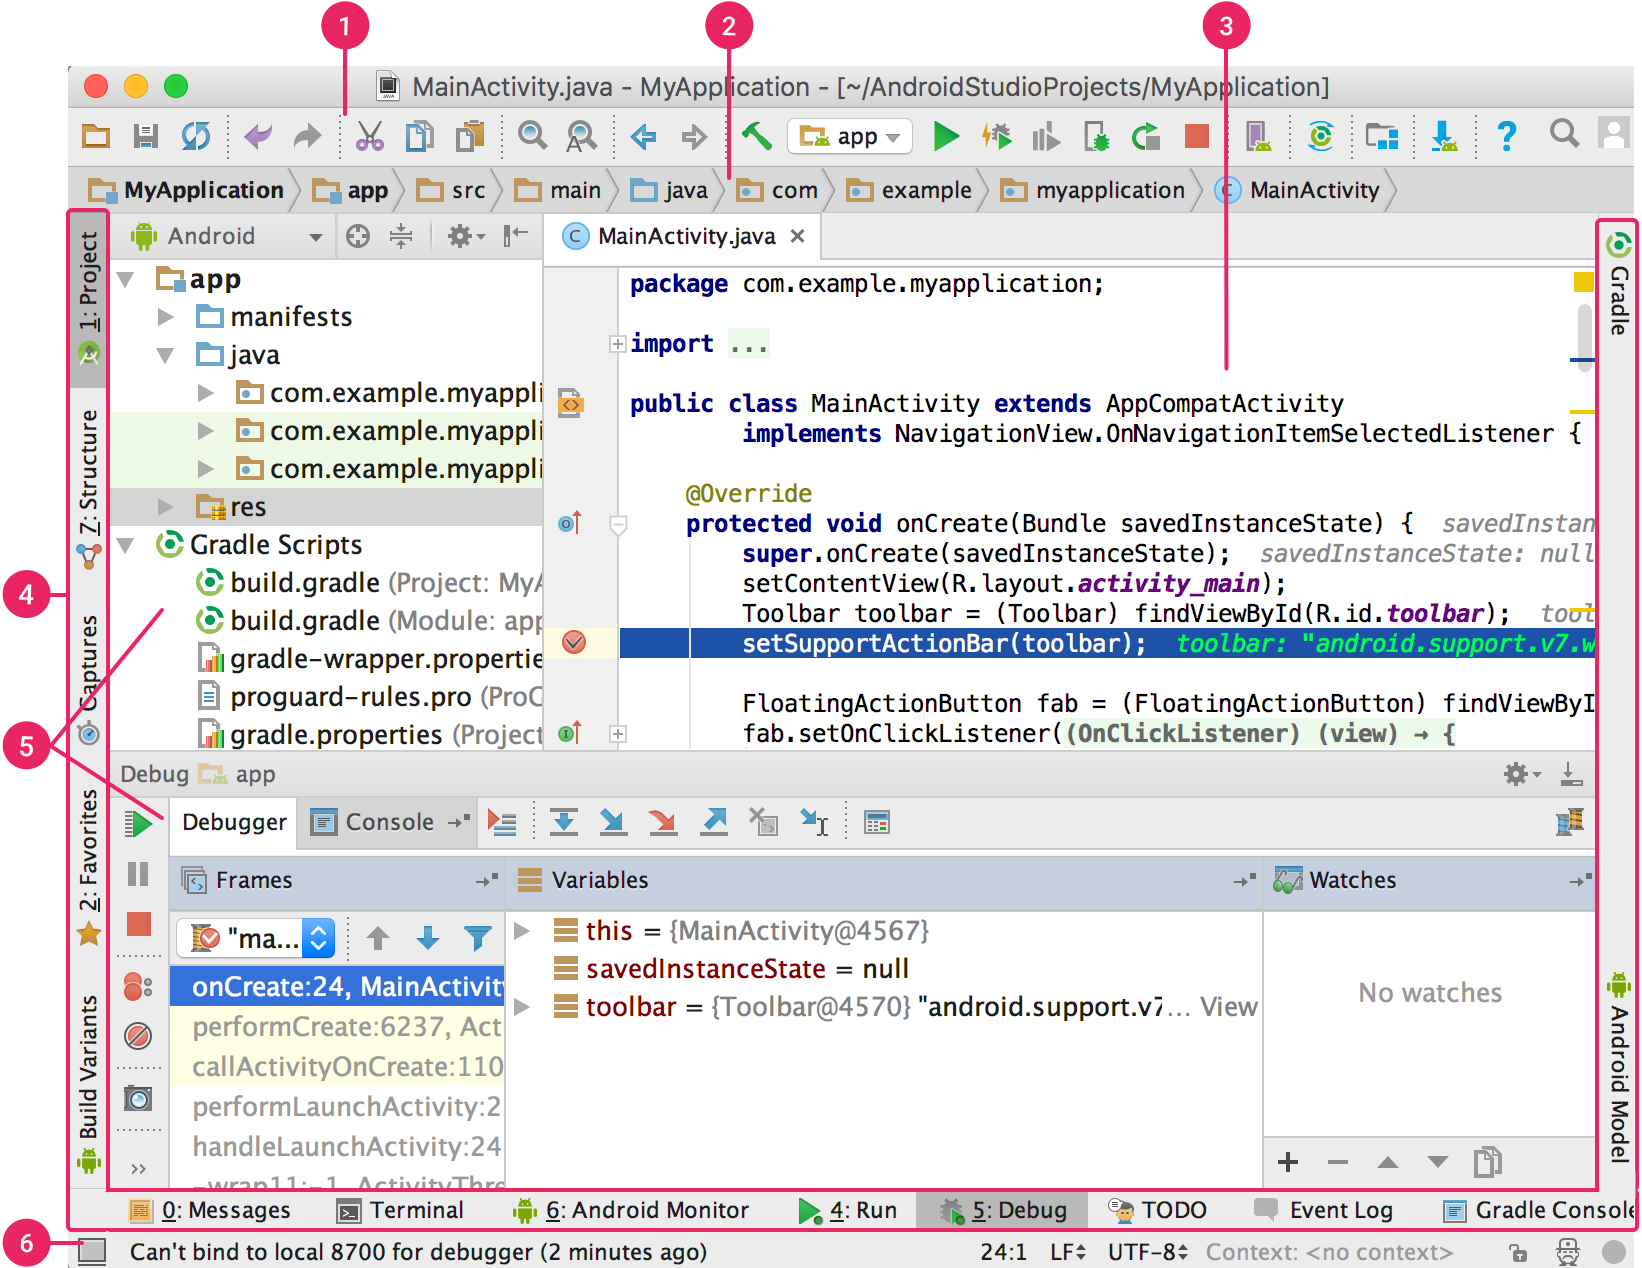
\includegraphics[scale=0.21]{ventana_android_studio.png} 
\floatfoot{Figura 4. Ventana de Android Studio}
\end{figure}

\begin{enumerate}
\item La barra de herramientas te permite realizar una gran
 variedad de acciones, como la ejecución de tu app y el inicio
 de herramientas de Android.
\item La barra de navegación te ayuda a explorar tu 
proyecto y abrir archivos para editar. Proporciona una 
vista más compacta de la estructura visible en la ventana Project.
\item La ventana del editor es el área donde puedes 
crear y modificar código. Según el tipo de archivo actual,
 el editor puede cambiar. Por ejemplo, cuando se visualiza
 un archivo de diseño, el editor muestra el editor de diseño.
\item La barra de la ventana de herramientas se extiende 
alrededor de la parte externa de la ventana del IDE y 
contiene los botones que te permiten expandir o contraer
 ventanas de herramientas individuales.
\item Las ventanas de herramientas te permiten acceder a 
tareas específicas, como la administración de proyectos,
 las búsquedas, los controles de versión, etc. Puedes 
expandirlas y contraerlas.
\item En la barra de estado, se muestra el estado de tu 
proyecto y del IDE en sí, como también cualquier advertencia 
o mensaje.
\end{enumerate}
\footnote{Fuente: Android Studio~\cite{ANDROIDSTUDIO}}
\section{Métodos}
En esta sección, vamos a listar una serie de métodos y buenas prácticas 
necesarias para este tipo de aplicación.
\subsection{Optimización de la batería del dispositivo}

En la mayoría de los casos, optimizar el uso de la batería de por parte de la aplicación es un tema secundario, pero en nuestro caso y debido a la necesidad de mantener el máximo tiempo posible emitiendo al dispositivo. Una hora más de emisión podría llegar a ser vital en el peor de los casos, ayudando incluso a salvar una vida, por lo que debemos mejorar todo lo posible este aspecto. Mejorar el rendimiento de la batería es un tema prioritario.


Para ello vamos a tener en cuenta tres aspectos importantes:
\begin{itemize}
\item Hacer una aplicación \textit{Lazy First}.
\item Utilizar las distintas características de la plataforma relacionadas con el consumo de batería.
\item Utilizar herramientas para encontrar la causa de la perdida de batería.
\end{itemize}

A continuación vamos a profundizar en cada uno de los aspectos anteriormente citados.
\subsubsection{Lazy First}

Hacer una aplicación Lazy First significa encontrar formas de reducir y optimizar operaciones que supongan una carga significativa para la carga de la batería. Las conceptos que deben aplicarse son los siguientes:
\begin{enumerate}
\item \textbf{Reducir:} Reducir el número de operaciones que se realizan, por ejemplo, utilizar una cache de datos descargados, en lugar de volver a descargarlos cada vez que los necesitemos.
\item \textbf{Aplazar:} Aplazar operaciones hasta que no supongan un impacto en la duración de la batería, por ejemplo, esperar a tener el cargador conectado para subir información al servidor.
\item \textbf{Agrupar:} Agrupar varias operaciones que puedan para que al realizarse de forma simultanea nos ahorre, por ejemplo, sacar el dispositivo de reposo varias veces.
\end{enumerate}

Deberemos utilizar estos principios cada vez que queramos utilizar la CPU, la antena, la pantalla o el GPS del dispositivo.
\subsubsection{Características de la plataforma}


La plataforma de Android nos ofrece mecanismos para conservar
 la vida de la batería. De forma que nos ofrece diversas APIs para
 planificar los procesos, describimos algunas en la sección de APIs~\cite{jobdispatcher}.

Dejando las APIs a un lado, caben destacar  dos funciones de
 ahorro de energía que presenta Android, ya que estas prolongan 
la vida de la batería administrando la forma en que las apps se 
comportan cuando un dispositivo no está conectado a una 
fuente de energía. Descanso reduce el consumo de batería
 aplazando la actividad de CPU y de red de las apps en segundo
 plano cuando el dispositivo no se usa durante períodos de
 tiempo prolongados. App Standby aplaza la actividad de red 
en segundo plano de las apps con las cuales el usuario no haya
 interactuado recientemente.

A continuación vamos a profundizar en ambas funciones.

\paragraph{Modo Descanso:}

Si un usuario deja un dispositivo desconectado, quieto y con la 
pantalla apagada durante un período de tiempo determinado, este 
entra en el modo Descanso. En el modo Descanso, el sistema intenta 
conservar la carga de la batería restringiendo el acceso por parte de
 las apps a servicios de uso intenso de red y CPU. También evita que
 las apps accedan a la red y aplaza sus tareas, sincronizaciones
 y alarmas estándares.

De forma periódica, el sistema desactiva el modo Descanso durante 
un tiempo breve para permitir que las apps completen sus actividades 
aplazadas. Durante este período de mantenimiento, el sistema ejecuta
 todas las sincronizaciones, tareas y alarmas pendientes, y permite 
que las apps accedan a la red.
\begin{figure}[h]
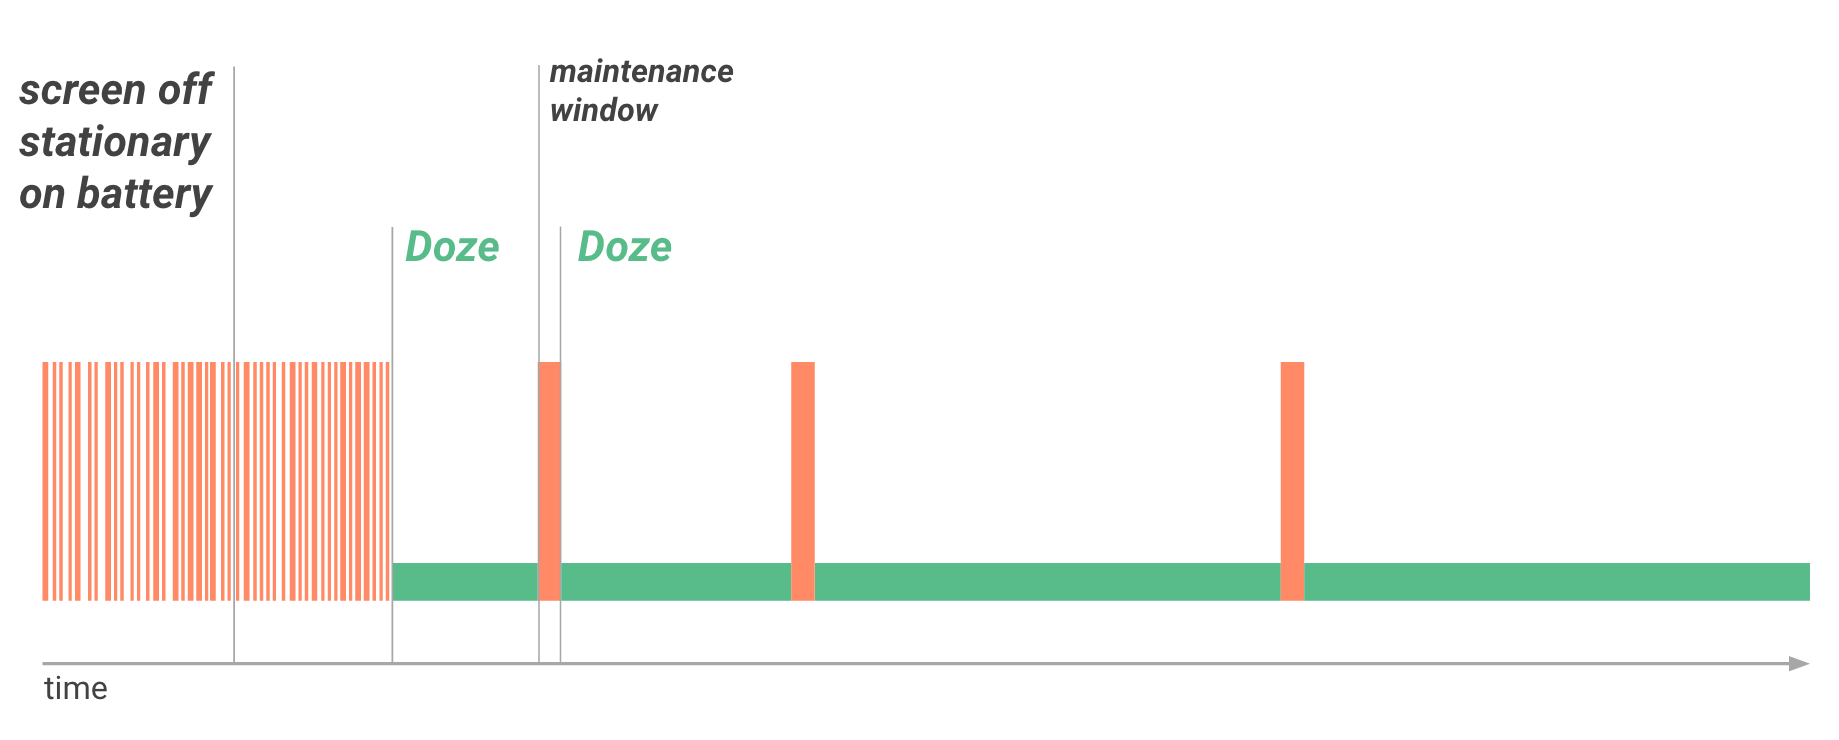
\includegraphics[scale=0.20]{imagenes/doze.png} 
\caption{Descanso proporciona un período de mantenimiento
 recurrente para que las apps usen la red y controlen actividades pendientes.}
\end{figure}



Al finalizar cada período de mantenimiento, el sistema vuelve a activar 
el modo Descanso, suspender el acceso a la red y aplazar tareas, 
sincronizaciones y alarmas. Con el paso del tiempo, el sistema programa
 los períodos de mantenimiento cada vez con menos frecuencia, lo cual
 permite reducir el consumo de batería en casos de inactividad durante 
más tiempo cuando el dispositivo no está conectado a un cargador.

Si bien el usuario activa el dispositivo moviéndolo, encendiendo la pantalla
 o conectándolo a un cargador, el sistema desactiva el modo Descanso 
y todas las apps vuelven a la actividad normal.

\paragraph{Restricciones del modo Descanso:}
Durante el modo Descanso, se aplican las siguientes restricciones a tus apps:
\begin{enumerate}
\item Se suspende el acceso a la red.
\item El sistema ignora los wake locks.
\item Las alarmas estándares AlarmManager (incluidas setExact() y setWindow())
 se aplazan hasta el siguiente período de mantenimiento.
\begin{enumerate}
\item Si necesitas programar alarmas que se activen en el modo Descanso, 
usa setAndAllowWhileIdle() o setExactAndAllowWhileIdle().
\item Las alarmas programadas con setAlarmClock() se activan con normalidad;
 el sistema desactiva el modo Descanso antes de que esas alarmas se activen.
\end{enumerate}
\item El sistema no realiza escaneos de Wi-Fi.
\item El sistema no permite que se ejecuten adaptadores de sincronización.
\item El sistema no permite que se ejecute JobScheduler.
\end{enumerate}

\paragraph{Información sobre App Standby}

El modo App Standby permite que el sistema determine si una app se
 encuentra inactiva cuando el usuario no la usa activamente. El sistema
 hace esta determinación cuando el usuario no aplica toques en la app
 durante un período determinado y cuando no rige ninguna de las 
siguientes condiciones:
\begin{enumerate}

\item El usuario inicia explícitamente la app.
\item La app actualmente tiene un proceso en primer plano 
(ya sea como actividad o como servicio en primer plano, o en uso por
 parte de otra actividad u otro servicio en primer plano).
\item La app genera una notificación que los usuarios ven en la pantalla 
bloqueada o en la bandeja de notificaciones.
\end{enumerate}

Cuando el usuario enchufa el dispositivo en una fuente de energía,
 el sistema libera las apps del estado de reposo, con lo cual les permite
 acceder libremente a la red y ejecutar cualquier tarea y sincronización
 pendientes. Si el dispositivo queda inactivo durante períodos prolongados, 
las apps inactivas pueden acceder a la red aproximadamente una vez al día.

\paragraph{Firebase Cloud Messaging}

Para poder utilizar nuestra aplicación en ambos modos de ahorro 
de batería utilizaremos la solución de mensajería 
 Firebase Cloud Messaging~\cite{FIREBASECLOUDMESS}, la cual nos
 permitirá enviar mensajes de forma segura al backend aún estando en 
ahorro de energía. Nos resultará sencilla su implementación al ya tener 
Firebase integrado en nuestra aplicación.

\subsubsection{Herramientas para analizar el consumo de batería}
Ahora vamos a listar un par de herramientas para Android que nos ayudarán a identificar las áreas en las que mejorar el consumo de batería. Utilizaremos estas herramientas para aplicar en estas áreas los principios de Lazy First.

\begin{enumerate}
\item \textbf{Profile GPU Rendering:} Esta herramienta nos mostrará, en forma de histograma de desplazamiento,una representación visual del tiempo necesario para representar los fotogramas de una ventana de IU en relación con un benchmark de 16 ms por fotograma.

En las GPU menos potentes, la frecuencia de relleno disponible (la velocidad a la cual la GPU puede rellenar el búfer de fotogramas) puede ser bastante baja. A medida que la aumenta la cantidad de píxeles requeridos para dibujar un fotograma, la GPU puede tardar más en procesar comandos nuevos y solicitar tiempo de espera al resto del sistema hasta ordenarse. La herramienta de generación de perfiles te ayuda a detectar los casos en que el rendimiento de la GPU se ve afectado cuando esta intenta dibujar píxeles o sobrecargado debido a una superposición voluminosa.
\item \textbf{Battery Historian:}Una útil herramienta para inspeccionar la relación entre la batería y los eventos de un dispositivo android, estando este apagado. Nos permitirá visualizar eventos de nivel de sistema y aplicación en una línea de tiempo para ver fácilmente varias estadísticas desde que se cargó el dispositivo por completo por última vez, es decir, podremos seleccionar nuestra aplicación y ver la evolución de la carga de la batería respecto a esta.\cite{BATTERYHISTORIAN}

\end{enumerate}
\footnote{Fuente: android developers \cite{OPTIMIZABATERIA}}
